\documentclass{beamer}
\usepackage{pifont}
\begin{document}

\title{Leveraging version control to accelerate research}

\graphicspath{{./figs}}
% ---------------------------------------------------------------------------%
\begin{frame}
  \maketitle

\end{frame}
% ---------------------------------------------------------------------------%

% ---------------------------------------------------------------------------%
\begin{frame}
  \tableofcontents
\end{frame}
% ---------------------------------------------------------------------------%


\section{Introduction}
% ---------------------------------------------------------------------------%
\begin{frame}{A note on terminology}
  Github $\subset$ git $\subset$ Version Tracking/Control $\subset$ Configuration Management
\end{frame}
% ---------------------------------------------------------------------------%

% ---------------------------------------------------------------------------%
\begin{frame}{Introduction to version control}
  \textbf{Version Control:} In software engineering, version control is a class of systems responsible for \textbf{managing changes to} computer programs, documents, large web sites, or other \textbf{collections of information.}
\only<2>{
  \begin{equation*}
    \downarrow
  \end{equation*}

  \textbf{Version control manages changes to collections of information.}}
\end{frame}
% ---------------------------------------------------------------------------%

% ---------------------------------------------------------------------------%
\begin{frame}{Introduction to version control}
  \begin{itemize}
  \item Broadly, version control allows you to:
    \begin{itemize}
    \item track, manage, and understand changes
    \item collaborate effectively
    \item store backups
    \item create and build upon ``known states''
    \end{itemize}
  \item Version control is often seen as a safety net, which may be why it is often ignored.
  \end{itemize}
\end{frame}
% ---------------------------------------------------------------------------%
\begin{frame}{Introduction to version control}
  \only<1>{
  However, version control can also accelerate progress!...Well, indirectly at least.}

  I will argue that effective utilization can
  \begin{itemize}
    \only<1->{
    \item \textbf{Reduce cognitive load}
      
    Utilizing \textbf{pull requests} and \textbf{branches} lowers cognitive overhead to start/continue one or multiple projects.}

  \only<2->{
  \item \textbf{Deliver incremental success}
    
    Working from a \textit{known state} towards a \textit{known state} allows for better project definitions, particularly when a task/project is ``done''}

  \only<3->{
  \item \textbf{Reduce technical debt}
    
    Standardized, automated, decentralized testing bakes in reproducibility, creates known states, and alerts you of unintentional changes.}

  \only<4->{
  \item \textbf{Bake in tenants of Open Science from the start}

    Building a ``product'' that is incrementally constructed, continuously tested, serving a well-defined goal, reduces work at the end of a project and makes your work easier to understand and build on top of.}
    
  \end{itemize}
\end{frame}
% ---------------------------------------------------------------------------%

\section{Git \& Github}
% ---------------------------------------------------------------------------%
\begin{frame}{Introduction to git}
  \begin{itemize}
  \item {\color{blue} \href{https://git-scm.com/book/en/v2/Getting-Started-A-Short-History-of-Git}{git was introduced in 2005 to manage development of the linux kernel.}}

  \item Extremely lightweight, pervasive, effectively manages projects of any size.

  \item There are plenty of ways to use git - I will show one that is probably sufficient.
  \end{itemize}
\end{frame}
% ---------------------------------------------------------------------------%

% ---------------------------------------------------------------------------%
\begin{frame}{Introduction to github}
  Github is:
  \begin{itemize}
  \item Perfect in almost every way \ding{51}
  \item ...owned by Microsoft \ding{55}
  \end{itemize}
\end{frame}
% ---------------------------------------------------------------------------%

% ---------------------------------------------------------------------------%
\begin{frame}{Introduction to github}
  Github is a cloud-based service that
  \begin{itemize}
  \item \textbf{is free for students} (and many others)
  \item \textbf{synchronizes git repositories}

    Collaborate with others or yourself, and/or deploy to cloud computing and/or HPC
    
  \item \textbf{integrates with many toolchains} I alluded to earlier (continuous integration, documentation, project management, etc)

  \item Has a wonderful {\color{blue} \href{https://docs.github.com/en/get-started/start-your-journey}{getting started tutorial}}
  \end{itemize}
\end{frame}
% ---------------------------------------------------------------------------%


% ---------------------------------------------------------------------------%
\begin{frame}{The git(hub) workflow \& branches}
    \begin{figure}
    \centering
    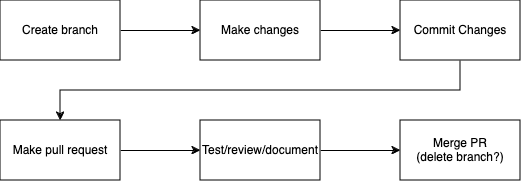
\includegraphics[width=\textwidth]{github_flow.png}
  \end{figure}

  \begin{itemize}
  \item \textbf{Branch}: An isolated environment to make changes in, without effecting other branches
  \item \textbf{Commit}: A single batch of changes, usually quite small
  \item \textbf{Pull Request}: (PR) A formal request to merge two branches, usually consisting of peer review/tests/documentation of changes
  \end{itemize}
\end{frame}
% ---------------------------------------------------------------------------%

% ---------------------------------------------------------------------------%
\begin{frame}{Use cases}
  \begin{itemize}
    \only<1>{
    \item \textbf{Branches}: topic branch, development branch, bug-fix, integration test}

    \only<2>{
    \item \textbf{Commits}: commits should happen frequently. Finish that function? Commit. Get another test to pass? Commit. Prove that theorem? Commit.}

    \only<3>{
  \item \textbf{Pull Requests}: PRs should happen when a coherent block of functionality is complete. Fix the bug you were hunting? Open a PR. Finish the task? Open a PR.

    \vspace{0.5cm}

    Further, PRs are a great place to document the state of the work and handle review comments. Add figures, justify the approach taken, document any hang ups and review comments/follow ups.}
  \end{itemize}
\end{frame}
% ---------------------------------------------------------------------------%

% ---------------------------------------------------------------------------%
\begin{frame}{Quick example}
  
\end{frame}
% ---------------------------------------------------------------------------%

% ---------------------------------------------------------------------------%
\begin{frame}{Github Actions}
  Github actions are configurable, automated scripts that
  \begin{itemize}
  \item run at pre-determined times (e.g., on PRs/merges)
  \item automate process like continuous integration (unit/integration testing), build and deploy documentation, codecoverage analysis, etc
  \item can post results in PRs upon completion
  \end{itemize}
  \vspace{0.5cm}
  
  Example: You develop on your laptop and use github to sync to the HPC. Use github actions to ensure your code builds in a clean linux environment.
  
  \vspace{0.5cm}
  
  \only<2>{\textbf{Github actions are \textit{powerful}}}
  
\end{frame}
% ---------------------------------------------------------------------------%

\section{Version Control \& Continuous Integration}
% ---------------------------------------------------------------------------%
\begin{frame}{}
  
\end{frame}
% ---------------------------------------------------------------------------%

\section{Test-Driven Development (or hypothesis-driven science)}
% ---------------------------------------------------------------------------%
\begin{frame}{}
  
\end{frame}
% ---------------------------------------------------------------------------%


\section{Bonus: Github Projects}
% ---------------------------------------------------------------------------%
\begin{frame}{}
  
\end{frame}
% ---------------------------------------------------------------------------%

\end{document}
